% The purpose of this chapter is to lay a foundation for understanding the technical choices made in the following chapters.
\chapter{Theory}
\label{chap:theory}
\section{Database management system}

A database is a set of data held in computer storage, often structured for rapid retrieval and modification. Applications interact with their database through a \acrfull{DBMS}.

A constantly increasing part of the world's population is gaining access to the internet. To accommodate this rapid growth, a matching increase in performance and ease of use is desired. The number of requests large scale applications experience can in extreme cases reach millions of write operations per second\cite[p.~43]{nosql-ntnu}. Developer expectations of databases has altered to accommodate such use cases by adopting new paradigms. 

\subsection{Distributed database}

Distribution is a paradigm for handling throughput larger than a single server can handle. Distributed databases consists of a network of physically separated computers and a system for maintaining the integrity of the database across multiple computers\cite[p.~4]{ddms}. This enables the database system to distribute the load over each machine, preferably to a computer physically near the client to ensure data localisation. Distributed databases have an advantage in performance and fault tolerance\cite[pp.~12--15]{ddms}.

\subsection{Document-oriented database}

Databases traditionally model relationships between data. These kinds of databases are called relational databases and a \acrfull{RDBMS} is used to enforce certain constraints on the data and the relationships between them. \acrshort{RDBMS} are advantageous in ensuring well-formed data and validating queries. However there are problems with this approach for some use cases. \acrshort{NoSQL}, of which document-oriented databases are a type, gives up on relational data and its advantages. However one can freely store data whose structure is not known in advance, as is commonly the case in big data. Like distributed databases it also comes with increased performance\cite{cmp-nosql} as there is simply less work for the database to do.

Document-oriented databases associate keys with structured data referred to as documents. The documents are usually stored in a standardised format like \acrshort{XML} or \acrshort{JSON}\cite[p.~9]{nosql-ntnu}. The document schemes are not constrained, and as such document-oriented databases fall under the \acrshort{NoSQL} category.

\section{Reactive programming}
Reactive programming is a paradigm applicable when continuous updates of information is preferred. Data that would traditionally be thought of as single data point is thought of as a stream of points over time in reactive programming. Streams can be transformed and combined to form new streams analogous to how cells in a spreadsheet depend on and update each other. Reactive programming enables elegant propagation of change throughout the domain.

\section{Continuous Integration}
Continuous Integration helps developers prevent integration problems, applies quality control and reduces delivery time. The main goal of \gls{CI} is to detect and correct errors in the code base early and make them easier to handle. This is done through two key aspects: (1) forcing developers to commit their changes daily, and (2) giving the developers swift feedback by running automatic tests on the build after committing changes. (1) makes the updates smaller and manageable, and (2) ensures that the results are deployable. \acrshort{CI} makes it easier to work incrementally and by extension more agile.

Most of these benefits are based on assumptions in the development community, and there are few peer-reviewed articles either proving or disproving these claims. This may be because the claims are hard to test, or there is little interest in the scientific community to answer these questions. However case studies from corporations seem to agree with most of these claims. These studies should not necessarily be viewed as scientific, as they are not peer-reviewed. Yet one of the few scientific articles on the subject suggests that \acrshort{CI} does in fact increase the amount of releases. Michael Hilton et al. found that introducing \acrshort{CI} to a project would on average more than double its release rate.

\pagebreak[4]
\section{Continuous Delivery}
Continuous Delivery is an evolution of Continuous Integration. \acrshort{CD} is based on making sure the build is deployment-ready at any given time. In automating the build, testing and deployment phase, one hopes to completely eliminate the week to months long process of getting a software product deployed\cite{continuousdeliveryfaster}.   

\begin{figure}[h!]
  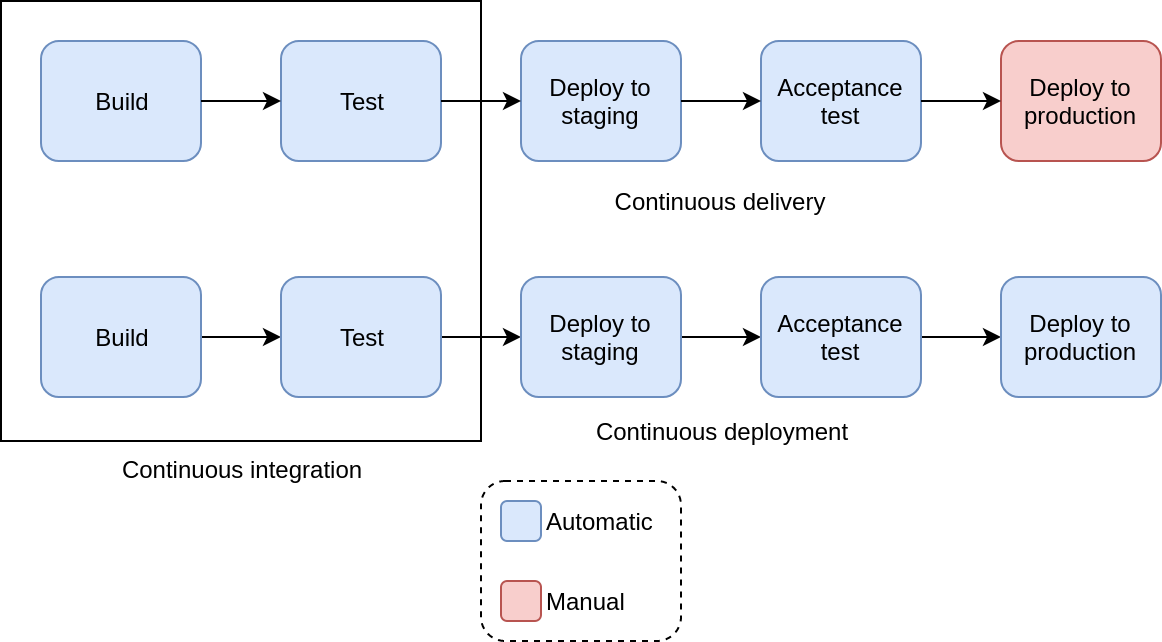
\includegraphics[width=\linewidth,height=\textheight,keepaspectratio]{images/ci_cd_comparison.png}
  \caption{CI/CD comparison}
  \label{fig:CI/CD-comparison}
\end{figure}

The advantages of \acrshort{CD} benefit corporations more than just in throughput and profitability. They increase employee satisfaction, which in turn increases worker productivity\cite{happy}.

\begin{displayquote}\textit{
    Firms with high-performing IT organisations were twice as likely to exceed their profitability, market share and productivity goals.
    High performers achieved higher levels of both throughput and stability.
    The use of continuous delivery practices including version control, continuous integration, and test automation predicts higher IT performance.
    Culture is measurable and predicts job satisfaction and organisational performance.
    Continuous Delivery measurably reduces both deployment pain and team burnout\cite{forsgren}.}
\end{displayquote}

\pagebreak[4]
\section{Security}
While \textit{attack vector} does not have a definition, in the nomenclature of computer security an attack vector usually refers to the path or mechanism by which a system is exploited or otherwise gained unauthorised access to\cite{av1}\cite{av2}\cite{av3}.

The sum of every possible attack vector constructs the \textit{attack surface} of a system. It follows that minimising the attack surface is desirable\cite[p.~1]{as} in a security context. The security community is working on quantitatively measuring the attack surface of a system. Intuitively one might measure the attack surface through the naive methods:

\begin{wraptable}{r}{7.65cm}
    \vspace{-2cm}
    \begin{tabularx}{7.65cm}{| X | c |}
        \hline
        \textbf{Attack class}                  & \textbf{Payoff}\\ \hline \hline
        httpd-module                           & .3\\ \hline
        open\_TCP/UDP-socket                   & .3\\ \hline
        world-accessible\_TCP/UDP-socket       & .4\\ \hline
        open\_unsecured\_env-mgmt              & .6\\ \hline
        open\_secured\_env-mgmt                & .2\\ \hline
        world\_accessible\_secured\_env-mgmt   & .3\\ \hline
        third-party\_credentials               & 1 \\ \hline
        world-accessible\_deployment-trigger   & .6\\ \hline
        locally-accessible\_deployment-trigger & .4\\ \hline
    \end{tabularx}
    \caption{The attack classes and their payoffs.}
    \label{fig:payoff}
\end{wraptable}

\begin{enumerate}
    \item Counting the number of bugs.
    \item Tracking known vulnerabilities.
\end{enumerate}

However Manadhata et al.\cite{as} suggests (1) is dependent on bug discovery. The process may miss or have false positive bugs, and it assigns equal severity to all bugs. (2) does not account for the system's configuration nor does the model capture future attackability. Manadhata et al. define\cite{as} a method for measuring an attack surface that they view as "meaningful and practical". By applying their method, a set of attack classes common for \acrshort{CD} tools can be built from the type hierarchy seen in figure \ref{fig:th}. These attack classes are assigned payoffs, seen in table \ref{fig:payoff}, with the method described in section \ref{sec:sciencemethod}. 

\begin{figure}[h]
\makebox[\textwidth][c]{
\begin{tikzpicture}[]
  \begin{scope}
    [tree layout,level distance=10mm,text depth=.1em,text height=.8em, every node/.append style={font=\small}]
    \graph[fresh nodes] {
        all resources <- {
            channel <- {
                TCP or UDP socket <- {
                    world accessible,
                    open
                }
            },
            credentials <- third party trust,
            deployment trigger <- {
                locally accessible,
                world accessible
            },
            httpd module,
            environment management <- {
                unsecured <- {
                    open,
                },
                secured <- {
                    world accessible,
                    open,
                }
            }
        }
    };
  \end{scope}
\end{tikzpicture}
}
\caption{Type hierarchy of the properties in the CD domain}
\medskip
\small
\centering 
Leaf nodes represent attack classes\footnotemark.
\label{fig:th}
\end{figure}

\pagebreak[3]
A minimal \acrshort{CD} solution that delivers the benefits expected has to at least implement the following:

\begin{itemize}
    \item \textbf{Deployment trigger}: The \acrshort{CD} solution needs to know when a new build of an application in the \acrshort{CD} system is available, so that the new build can be processed and delivered to the environments.
    \item \textbf{Delivery to environments}: Delivering a build of an application to an environment requires the environment to have a management \acrshort{API}. The \acrshort{API} must at least allow the actions: (1) shutting down a running instance of the application, and (2) start a new instance with the executable contents of the new build. The \acrshort{CD} solution needs privileges to perform both actions.
\end{itemize}


The features of a minimal \acrshort{CD} solution necessarily increases the \textit{attack surface} by introducing the following \textit{attack vectors}:
\begin{itemize}
    \item The \textit{deployment trigger} needs to open a \acrshort{TCP} or \acrshort{UDP} socket to the system that signals when a new build is ready. In a typical setup a \acrshort{CI} system would build and test a new version of an application, then send a trigger to the \acrshort{CD} solution
    \item For the \acrshort{CD} system to \textit{deliver} to environments it needs a credential for each environment that identifies it and grants the necessary privileges
    \item The \acrshort{CD} solution also needs to open a \acrshort{TCP} or \acrshort{UDP} socket to communicate with the environment \acrshort{API}
\end{itemize}

\footnotetext{This figure is based on the type hierarchy example\cite{as} presented in the article by Manadhata et al.}

The attack classes identified from the type hierarchy in figure \ref{fig:th} are described below:

\textbf{httpd-module}: \begin{displayquote}
"\textit{This attack class consists of all resources of type \textbf{httpd\_module}. CAN-2003-0789 describes a vulnerability  involving  handling  of  CGI  redirect  in  the \textbf{mod\_cgid} module in \textbf{apache} which an attacker can exploit to view sensitive information.}"\footnotemark[2]
\end{displayquote}

\pagebreak[1]
\textbf{open\_TCP/UDP-socket}: \begin{displayquote}
"\textit{The services  running  on  the system open TCP/UDP sockets and listen for client requests on them. Multiple sockets can be opened by a service and multiple services can share the same socket. This attack class is a subtype of the resource type channel. CVE-2001-0309 describes an attack involving open sockets since the \textbf{inetd} daemon does not properly close sockets for internal services such as \textbf{daytime} and \textbf{echo}, an attacker can cause a denial-of-service attack by opening a series of connections to these services.}"\footnotemark[2]
\end{displayquote}

\footnotetext[2]{Quote taken from Manadhata et al.\cite{as}}

\pagebreak[2]
\textbf{world-accessible\_TCP/UDP-socket}: \begin{displayquote}
This attack class derives from the \textit{open\_TCP/UDP-socket} attack class, however it being accessible by anyone who knows the address increases the risk associated. It opens for the possibility of distributed denial-of-service attacks\cite{ddos}.
\end{displayquote}

\pagebreak[2]
\textbf{open\_unsecured\_env-mgmt}: \begin{displayquote}
An integral part of \acrshort{CD} is the automatic deployment of programs to environments that run a class of programs. The environments needs to provide an \acrshort{API} the \acrshort{CD} solution can use to create and restart programs on certain triggers. This \acrshort{API} provides attackers with free reign to manipulate programs in the environments if they get access to the network. 
\end{displayquote}

\pagebreak[2]
\textbf{open\_secured\_env-mgmt}: \begin{displayquote}
Like \textit{open\_unsecured\_env-mgmt} this class exposes an \acrshort{API} for attackers, however the \acrshort{API} is secured by TLS certificates, the \acrshort{CD} is identified with a certificate signed by the environment. Certificates significantly reduce, but does not eliminate, the attackability of the \acrshort{API}. RFC7457\cite{rfc7457} summarises known attacks, as such the possibility of future attacks is present.
\end{displayquote}

\pagebreak[2]
\textbf{world\_accessible\_secured\_env-mgmt}: \begin{displayquote}
This attack class is very similar to \textit{open\_secured\_env-mgmt}. Exposing a TLS protected management \acrshort{API} to the world is not a big concern as TLS is in widespread use identifying owners of domains by website owners\cite{sslpulse}, and has proven itself not to be an easy target. However it does somewhat increase the associated risk compared to the \textit{open\_secured\_env-mgmt} class.
\end{displayquote}

\pagebreak[2]
\textbf{third-party\_credentials}: \begin{displayquote}
Since the \acrshort{CD} solution requires access to the environment \acrshort{API} an attacker could compromise the \acrshort{CD} solution itself and gain access to the environment \acrshort{API} through the \acrshort{CD} tool. The certificate could also possibly be misused by the third party.
\end{displayquote}

\pagebreak[2]
\textbf{world-accessible\_deployment-trigger}: \begin{displayquote}
As part of a larger system, \acrshort{CD} solutions often deploy based on external triggers. An attacker could fake such an external trigger, especially when some external triggers don't support any kind of identification or encryption.\cite{docker-no-id}
\end{displayquote}

\pagebreak[2]
\textbf{locally-accessible\_deployment-trigger}: \begin{displayquote}
Like \textit{world-accessible\_deployment-trigger}, but is only exposed on the internal network. 
\end{displayquote}